\section{Physics improvements for photon interactions}

\begin{figure}
	\centering
    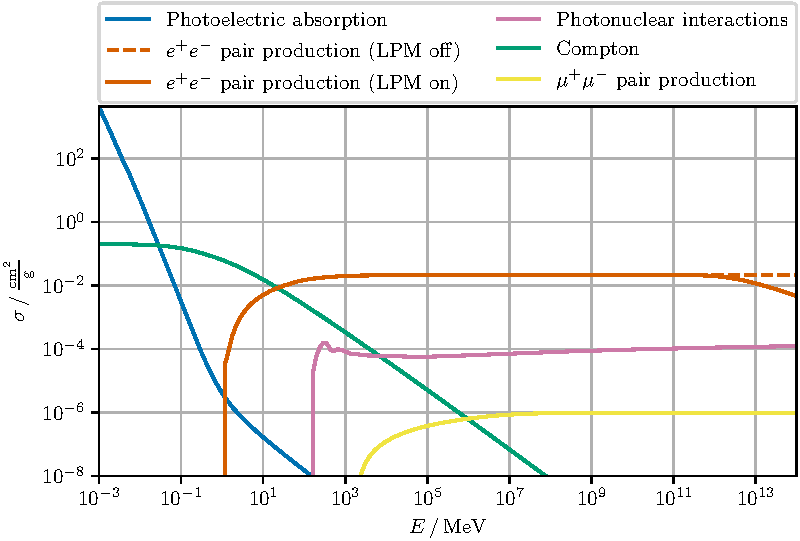
\includegraphics{plots/Photon_Air_dndx_ecut_0.pdf}
    \caption{Total cross section of photons in air inside PROPOSAL.}
    \label{fig:total_cross_photon}
\end{figure}


\subsection{Photoelectric absorption}

Photoelectric absorption describes the ejection of an atomic electron due to its interaction with an in-going photon.
In this process, the photon energy is used to free the electron from its atomic binding, while the remaining photon energy serves as the kinetic energy of the now free electron.
For photons in air, photoelectric absorption becomes the dominant interaction process for energies below $\approx \SI{30}{\kilo\electronvolt}$.
In the context of electromagnetic cascades, photoelectric absorption as a process starts to become important for energies where its cross section represents a significant correction to the total mean free path length.

The detailed description of photoelectric absorption is non-trivial and dependent on the properties of the atomic structure of the interaction target.
Since other codes to describe these processes already exist, PROPOSAL only provides an approximate description based on the cross section given in \cite{heitler, sauter}.
The total cross section is defined as
%
\begin{align}
	\label{eqn:sauter}
	\sigma &= 4 \pi r_e^2 Z^5 \alpha^4 F_1 F_2 \left( \frac{m_e}{E} \right)^5 \left( \gamma^2 -1 \right)^{\sfrac{3}{2}} \left[ \frac{4}{3} + \frac{\gamma (\gamma - 2)}{\gamma + 1} \left( 1 - \frac{\ln{\left( \gamma + \sqrt{\gamma^2 - 1} \right)}}{\gamma \sqrt{\gamma^2 - 1}}  \right) \right],
\end{align}
%
with the photon energy $E$ and the definitions
\begin{align}
	\gamma &= 1 + \frac{E - I}{m_e}, & I &= \frac{Z^2 \alpha^2 m_e}{2}.
\end{align}
%
The term
\begin{align}
	F_1 &= \left[ 1 + \left( \frac{\alpha Z}{\beta} \right)^2 \right] \frac{\pi \alpha Z / \beta }{\sinh(\pi \alpha Z / \beta )} \exp\left[ \frac{\alpha Z}{\beta} \left( \pi - 4 \arctan\left( \frac{\beta}{\alpha Z} \right) \right) \right]
\end{align}
%
is used as a correction factor for the non-relativistic energy regime \cite{sauter}, while the term
%
\begin{align}
	F_2 &= 1 + 0.01481 \ln^2{Z} - 0.000788 \ln^3{Z}
\end{align}
%
is an empirical correction describing the ratio between the K-shell and total photoelectric absorption cross section \cite{hubbell1969}.

The photoelectric cross section and a validation of the total photon cross section at low energies is shown in Figure \ref{fig:photoeffect_nist}, where the total photon cross section in air is compared to the calculations from the NIST Standard Reference Database.
The agreement is at worst \SI{10}{\percent}.

\begin{figure}
	\centering
    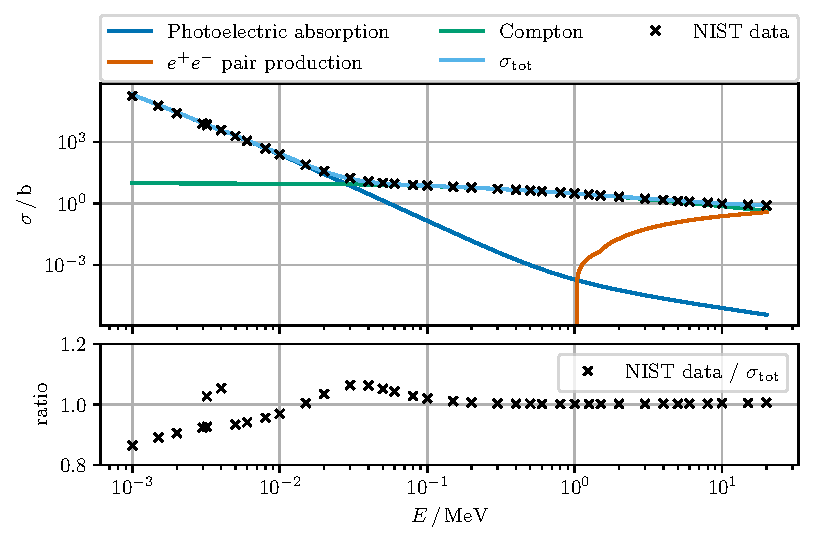
\includegraphics{plots/photoeffect_nist.pdf}
    \caption{Photon cross sections in air for small energies, compared to the total cross section according to the NIST Standard Reference Database.}
    \label{fig:photoeffect_nist}
\end{figure}

\subsection{Photonuclear interactions}


\begin{align}
	\label{eqn:photonuclear_C7}
	\sigma_{\gamma,N} &=
	\begin{cases}
		\left(73.3 s^{0.073} + 191.7 s^{-0.602} \right) \sqrt{1 - s_0 / s} \si{\micro\barn}, & \text{for } \sqrt{s} \leq \SI{19.39}{\giga\electronvolt}, \\
		\left( 59.3 s^{0.093} + 120.2 s^{-0.358} \right) \si{\micro\barn}, & \text{for } \sqrt{s} > \SI{19.39}{\giga\electronvolt}, \\
	\end{cases}
\end{align} 

with the squared center of mass energy $s = m_n^2 + 2 m_n \nu$ and the pion production threshold $\sqrt{s_0} = \SI{1.0761}{\giga\electronvolt}$.

\todo{Shadowing???}

\begin{figure}
	\centering
    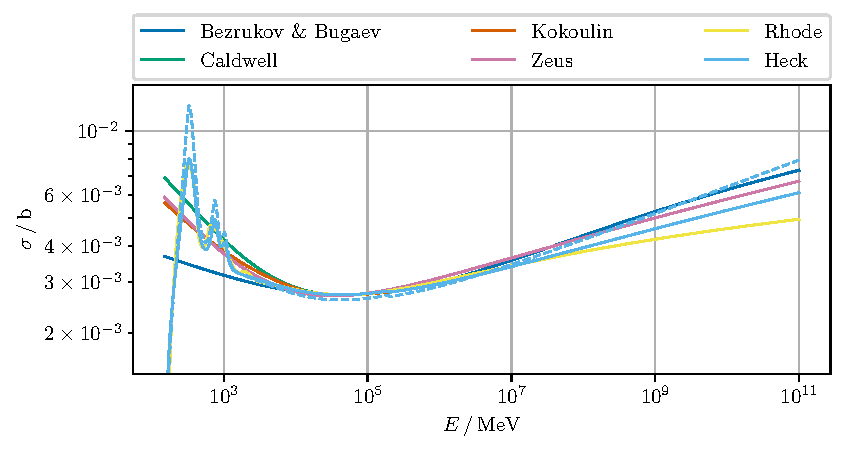
\includegraphics{plots/photoproduction_cross.pdf}
    \caption{Photonuclear interaction cross sections.}
    \label{fig:photoproduction_cross}
\end{figure}


\subsection{Muon pair production}

\begin{align}
	\frac{\mathrm{d}\sigma}{\mathrm{d}x} &= 4 Z^2 \alpha \left( r_e \frac{m_e}{m_\mu} \right)^2 \Phi(\delta) \left[ 1 - \frac{4}{3} (x - x^2) \right],
\end{align}
%
with
%
\begin{align}
	\Phi(\delta) &= \underbrace{\ln \left( \frac{B Z^{\sfrac{-1}{3}} m_\mu / m_e}{1 + B Z^{\sfrac{-1}{3}} \sqrt{e} \delta / m_e } \right)}_{\Phi_0} - \underbrace{\ln\left( \frac{D_n}{1 + \delta (D_n \sqrt{e} - 2) / m_\mu} \right)}_{\Delta_\text{n}},
\end{align}
%
where
%
\begin{align}
	x &= \frac{E_{\mu^-}}{E}, & \delta &= \frac{m_\mu^2}{2 E x (1 - x)}, & D_n &= 1.54 A^{0.27}.
\end{align}
%

\begin{align}
	\Phi(\delta) &\rightarrow \Phi(\delta) + \frac{1}{Z} \left[ \ln\left( \frac{m_\mu / \delta}{\delta m_\mu / m_e^2 + \sqrt{e}} \right) - \ln\left( 1 + \frac{1}{\delta \sqrt{e} B^\prime Z^{\sfrac{-2}{3}} / m_e} \right) \right]
\end{align}

For $Z > 1$, the effect of the inelastic nuclear form factor is taken into account by substituting
%
\begin{align}
	\Delta_\text{n} &\rightarrow \left( 1 - \frac{1}{Z} \right) \Delta_\text{n}.
\end{align}

\subsection{Landau-Pomeranchuk-Migdal effect}

\begin{align}
	\label{eqn:lpm_photopair}
	\frac{\mathrm{d}\sigma_\text{LPM}}{\mathrm{d}x} &= \frac{\mathrm{d}\sigma}{\mathrm{d}x} \cdot \frac{\xi(s) / 3 \left(G(s) + 2 \left( x^2 + (1 - x)^2 \right) \phi(s) \right)}{1 - 4 / 3 x (1 - x)},
\end{align}

\begin{align}
	\phi(s) &=
	\begin{cases}
		1 - \exp{\left\{ -6s \left(1 + (3 - \pi) s\right) + \frac{s^3}{ 0.623 + 0.796s + 0.658 s^2} \right\}} & \text{if $s < \num{1.54954}$}, \\
		1 - 0.012 s^{-4} & \text{if $s \geq \num{1.54954}$},
	\end{cases}
\end{align}
%
\begin{align}
	G(s) &=
	\begin{cases}
		3\psi(s) - 2\phi(s) & \text{if $s < \num{0.710390}$}, \\
		36s^2 / \left(36s^2 + 1 \right) & \text{if $\num{0.710390} \leq s < \num{0.904912}$}, \\
		1 - 0.022s^{-4} & \text{if $s \geq \num{0.904912}$},
	\end{cases}
\end{align}
%
\begin{align}
	\psi(s) &= 1 - \exp{\left\{ -4s - \frac{8s^2}{1 + 3.936s + 4.97s^2 - 0.05s^3 + 7.5 s^4} \right\}},
\end{align}
%
\begin{align}
	\xi(s) &\approx \xi(s^\prime) =
	\begin{cases}
		2 & \text{if $s^\prime < s_1$}, \\
		1 + h - \frac{0.08 (1 - h) (1 - (1-h)^2)}{\ln{(s_1)}} & \text{if $s_1 \leq s^\prime < 1$}, \\
		1 & \text{if $s^\prime \geq 1$},
	\end{cases}
\end{align}


\begin{align}
	s &= \frac{s^\prime}{\sqrt{\xi(s^\prime)}}, & s^\prime &= \frac{1}{8} \sqrt{\frac{E_\text{LPM}}{E x ( 1 - x)}}, & s_1 &= \frac{\sqrt{2} Z^{\sfrac{2}{3}}}{B^2}, \\ E_\text{LPM} &= \frac{2 \alpha (m_e c^2)^2 X_0}{\pi \hbar c}, & h &= \frac{\ln{(s^\prime)}}{\ln{(s_1)}}, & D_n &= 1.54 A^{0.27},
\end{align}

\begin{figure}
\centering
\begin{minipage}[t]{.48\textwidth}
  \centering
  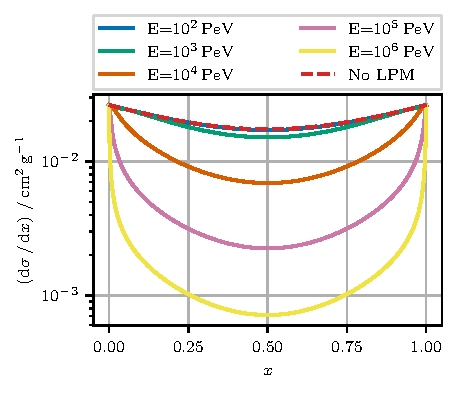
\includegraphics{plots/lpm_photopair_differential_small.pdf}
  \captionof{figure}{Differential cross section for electron-positron pair production in air at standard density, with nitrogen as an interaction target. The effect of the LPM effect at different energies is shown. Note that without the LPM suppression, the differential cross section is identical for all energies in this plot.}
  \label{fig:lpm_photopair_diff}
\end{minipage}%
\hfill
\begin{minipage}[t]{.48\textwidth}
  \centering
  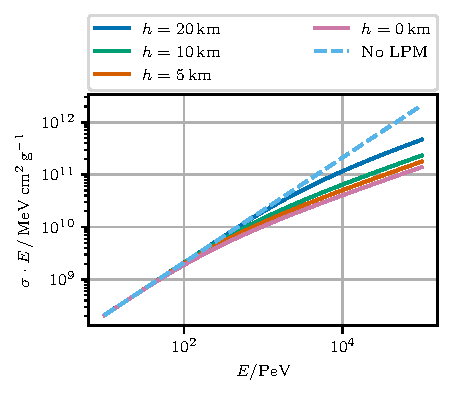
\includegraphics{plots/lpm_cross_photopair_small.pdf}
  \captionof{figure}{Total cross section for electron-positron pair production in air, with the effect of the LPM suppression at different atmospheric heights.}
  \label{fig:lpm_photopair_cross}
\end{minipage}
\end{figure}